\documentclass[conference]{IEEEtran}
\IEEEoverridecommandlockouts
\usepackage{cite}
\usepackage{amsmath,amssymb,amsfonts}
\usepackage{algorithmic}
\usepackage{graphicx}
\usepackage{textcomp}
\usepackage{xcolor}
\usepackage{url}

\def\BibTeX{{\rm B\kern-.05em{\sc i\kern-.025em b}\kern-.08em
    T\kern-.1667em\lower.7ex\hbox{E}\kern-.125emX}}

\begin{document}

\title{On the Reliability of Targeted Unlearning in 4-Bit Quantized LLMs}

\author{
\IEEEauthorblockN{Syed Ahsan Ali}
\IEEEauthorblockA{
NED University of Engineering and Technology \\
Karachi, Pakistan \\
Email: mrahsanali5@gmail.com \\
ORCID: 0009-0002-3763-929X
}
}

\maketitle

\begin{abstract}
Large language model unlearning is typically evaluated in high-resource settings, while real-world deployments increasingly rely on memory-efficient pipelines such as 4-bit quantization and parameter-efficient fine-tuning (PEFT). This raises a key question: whether targeted unlearning remains reliable, secure, and privacy-preserving under such deployment constraints. This paper evaluates the dependability of targeted unlearning under a 4-bit quantized LLaMA-3 pipeline using TOFU and membership inference analysis across three random seeds.

Three practical strategies are studied: Pure Gradient Ascent (PGA), retention-regularized Gradient Ascent (GAFT), and IDK-based supervised refusal tuning. The multi-seed results show that different unlearning strategies induce substantially different privacy-utility trade-offs. GAFT provides the most reliable balance across forgetting and privacy signals, IDK achieves stronger direct suppression of memorized knowledge and the lowest MIA scores, and PGA exhibits comparatively unstable behavior under the same quantized setup.

These findings suggest that unlearning effectiveness observed in idealized settings may not directly translate to dependable deployment scenarios, motivating system-level evaluation of unlearning in deployed ML systems.
\end{abstract}

\renewcommand\IEEEkeywordsname{Keywords}
\begin{IEEEkeywords}
\textit{Machine Unlearning, Large Language Models, Quantized LLMs, TOFU Benchmark, Membership Inference Attack, Privacy-Utility Trade-off, AI Security}
\end{IEEEkeywords}

\section{Introduction}
Machine unlearning has become a key requirement for deploying large language models (LLMs) in privacy-sensitive environments. As users and regulators increasingly demand deletion or suppression of specific knowledge, model developers need practical methods to remove targeted information without retraining from scratch. At the same time, most real-world LLM deployments now rely on memory-efficient settings, such as low-bit quantization and parameter-efficient fine-tuning (PEFT), where unlearning behavior is still not well understood. In deployed generative AI systems, this is not only a modeling question but also a dependability and security question, because privacy leakage, unstable forgetting, and deployment-induced failures can propagate across system boundaries.

Targeted unlearning in LLMs is also difficult to define and evaluate precisely. In autoregressive models, forgetting should not be interpreted as guaranteed semantic erasure of every fact related to an entity, because relevant information may remain distributed across parameters, surface through paraphrases, or reappear as hallucinated substitutions. Likewise, a model that no longer reproduces the original answer verbatim may still reveal residual evidence of training exposure through privacy attacks. For this reason, practical unlearning in deployed LLMs should be treated as a multi-objective problem spanning forget-set suppression, retained utility, and privacy leakage rather than as a single benchmark score.

This paper investigates whether targeted unlearning remains dependable when deployed under memory-efficient constraints such as 4-bit quantization and LoRA-based fine-tuning.

While prior work has extensively studied unlearning in full-precision settings, relatively little attention has been given to its behavior under quantized deployment pipelines. This creates a gap between research assumptions and real-world usage. We frame unlearning as a reliability and privacy problem in deployed ML systems, where privacy leakage, robustness, system-level evaluation, and deployment constraints must be evaluated jointly rather than treated as secondary concerns.

In this paper, we present an empirical study of targeted unlearning in a 4-bit quantized LLM using the Unsloth training framework [14] and the TOFU benchmark. We compare three practical strategies: (i) Pure Gradient Ascent, (ii) retention-regularized Gradient Ascent (GAFT), and (iii) IDK-based supervised refusal tuning. We evaluate them using TOFU-based forgetting and retention metrics and complement this analysis with membership inference attack (MIA) signals to assess residual privacy leakage under deployment constraints. To improve robustness relative to an initial single-seed protocol, we repeat each method with three random seeds and report aggregate statistics across runs.

Our experiments show that unlearning quality depends strongly on the optimization objective: pure gradient ascent is less stable, IDK tuning improves direct suppression and privacy, and GAFT provides a stronger overall balance between forgetting and retained utility in our setting. These findings highlight that practical unlearning in quantized LLMs should be assessed as a multi-objective reliability and security problem rather than a single-metric optimization.

Our contributions are:
\begin{itemize}
\item We evaluate targeted unlearning under a 4-bit quantized LLM pipeline, reflecting realistic deployment constraints.
\item We strengthen the empirical protocol by repeating each method with three random seeds and reporting aggregate variability rather than single-run point estimates.
\item We make the forgetting target explicit in an LLM setting by treating it as reduced reliance on a designated forget set while preserving retained and out-of-scope utility, rather than as unverifiable perfect semantic erasure.
\item We compare three unlearning strategies (PGA, GAFT, IDK) under a unified evaluation framework that combines benchmark metrics with privacy-oriented membership inference signals.
\item We show that unlearning behavior varies significantly across methods, raising concrete reliability and security concerns for low-resource deployment settings.
\end{itemize}

\section{Background and Related Work}
Machine unlearning in LLMs has emerged as a practical approach to removing the influence of targeted training examples without full retraining [1], [3]. Prior work has studied gradient-based unlearning, supervised target replacement, and multi-objective formulations that combine forgetting with utility preservation [2], [4], [5]. These studies establish the core problem setting, but most analyze behavior in comparatively idealized full-precision environments.

Parameter-efficient fine-tuning (PEFT), especially LoRA, is now central to practical LLM adaptation because it reduces memory and computation costs while preserving strong downstream performance [9]. Recent work suggests that PEFT-based unlearning can be effective and can improve the privacy-utility trade-off relative to naive updates [10]. At the same time, scaling-law analyses indicate that forgetting and retained utility are inherently coupled, which helps explain why aggressive forgetting objectives may become unstable [11].

Privacy evaluation is also a key part of the unlearning literature. Membership inference attacks (MIA) remain a standard way to test whether a model continues to reveal evidence of exposure to data that should be forgotten [7]. This concern is reinforced by memorization and extraction work showing that LLMs can retain and reveal training information even when simple behavioral evaluation suggests otherwise [8].

At the same time, recent LLM unlearning work has made clear that benchmark scores should be interpreted operationally rather than as proof of complete semantic deletion. Forget/retain splits define which examples should lose influence, but they do not by themselves certify that every semantically related fact has been removed. This motivates using multiple complementary signals, including retained utility and privacy-oriented attacks, when judging whether an unlearning method is dependable in practice [8], [13].

Quantization is particularly important in deployment settings. Prior work shows that low-bit quantization can substantially alter apparent unlearning effectiveness and, in some cases, recover supposedly forgotten knowledge after deployment transformations [12]. TOFU provides a controlled benchmark for studying these trade-offs under standardized forget/retain splits [13]. However, existing studies rarely evaluate targeted unlearning under fully quantized deployment pipelines, motivating the analysis in this work.

\section{Method}
\subsection{Problem Formulation}
Given a fine-tuned language model $f_{\theta}$, the objective of unlearning is to remove information associated with a target forget set $\mathcal{D}_f$ while preserving performance on a retain set $\mathcal{D}_r$. In our experiments, $\mathcal{D}_f$ corresponds to TOFU forget10 and $\mathcal{D}_r$ corresponds to TOFU retain90.

In this paper, the forgetting target is example-conditioned rather than ontology-level. That is, we do not ask whether the model has erased every semantically adjacent fact about an entity; instead, we ask whether the model's reliance on the designated TOFU forget examples can be reduced without causing broad collateral damage on retained and unrelated behavior. In the LLM setting, targeted forgetting is difficult to interpret as complete semantic erasure, since knowledge may be distributed across model parameters and expressed through paraphrases or related generations. Following prior TOFU-style unlearning work, we therefore adopt an operational definition of forgetting: after unlearning, the model should exhibit reduced reliance on information associated with the designated forget set $\mathcal{D}_f$, while preserving performance on the retain set $\mathcal{D}_r$ and on unrelated capabilities outside the unlearning scope. In this paper, successful forgetting is therefore assessed through forget-set suppression, retained utility, and privacy-oriented membership signals rather than through a claim of perfect removal of all semantically related knowledge.

The standard supervised objective minimizes cross-entropy over a dataset $\mathcal{D}$:
\begin{equation}
\mathcal{L}_{\mathrm{CE}}(\theta; \mathcal{D}) = -\frac{1}{|\mathcal{D}|}\sum_{(x,y)\in\mathcal{D}} \log p_{\theta}(y\mid x)
\end{equation}

Unlearning is then implemented by modifying this objective so that model updates move away from forget samples and, when required, remain aligned with retain samples.

\subsection{Pure Gradient Ascent (PGA)}
Pure Gradient Ascent provides the most direct unlearning intervention. Instead of minimizing loss on forget samples, it maximizes the forget loss:
\begin{equation}
\mathcal{L}_{\mathrm{PGA}}(\theta) = -\mathcal{L}_{\mathrm{CE}}(\theta; \mathcal{D}_f)
\end{equation}

Under gradient descent on $\mathcal{L}_{\mathrm{PGA}}$, the parameter update becomes:
\begin{equation}
\theta_{t+1} = \theta_t - \eta\nabla_{\theta}\mathcal{L}_{\mathrm{PGA}}(\theta_t) = \theta_t + \eta\nabla_{\theta}\mathcal{L}_{\mathrm{CE}}(\theta_t; \mathcal{D}_f)
\end{equation}

Intuitively, this pushes model parameters away from solutions that correctly reproduce target forget facts. The method is effective for aggressive forgetting, but because it does not explicitly preserve non-target knowledge, it can increase utility degradation risk.

\subsection{Gradient Ascent with Retain Constraint (GAFT)}
To reduce catastrophic forgetting, we use a mixed objective that combines forget ascent and retain descent:
\begin{equation}
\mathcal{L}_{\mathrm{GAFT}}(\theta) = -\mathcal{L}_{\mathrm{CE}}(\theta; \mathcal{D}_f) + \gamma\mathcal{L}_{\mathrm{CE}}(\theta; \mathcal{D}_r')
\end{equation}

Here, $\mathcal{D}_r'$ is a sampled retain subset and $\gamma$ controls the retain-preservation strength. In this work, $\gamma = 0.7$.

A custom mixed-factor batch sampler enforces a fixed batch composition (one forget + one retain sample for batch size 2). This design ensures that every update receives both a forgetting signal and a utility-preserving signal, leading to more stable optimization than unconstrained ascent.

\subsection{IDK Tuning}
IDK Tuning replaces original forget answers with an abstention response: ``I do not have that information.''

Let $\mathcal{D}_f^{\mathrm{idk}}$ denote the transformed forget set. The objective becomes:
\begin{equation}
\mathcal{L}_{\mathrm{IDK}}(\theta) = \mathcal{L}_{\mathrm{CE}}(\theta; \mathcal{D}_f^{\mathrm{idk}} \cup \mathcal{D}_r')
\end{equation}

Rather than forcing the model to become incorrect, this method encourages controlled abstention on sensitive targets while retaining normal behavior elsewhere. Conceptually, it acts as response-level unlearning through supervised re-alignment.

\subsection{Optimization and Implementation}
All methods are implemented in the same training stack (Unsloth [14] + TRL/HuggingFace), with method-specific loss definitions realized via custom trainer logic or transformed training targets. We use Unsloth for efficient 4-bit loading and LoRA-based fine-tuning in the memory-constrained training pipeline. This keeps the optimization pipeline consistent and makes comparisons methodologically fair. The model is loaded and fine-tuned directly in 4-bit precision, and all evaluations are performed on the same quantized model.

\section{Experimental Setup}
\subsection{Dataset and Splits}
We use the TOFU benchmark for controlled machine unlearning evaluation. The forget split is forget10, the retain split is retain90, and the full split is used for the initial memorization stage.

\subsection{Base Model and PEFT Configuration}
The base model is \texttt{unsloth/llama-3-8b-bnb-4bit}. To enable efficient adaptation, LoRA is applied with $r = 16$, $\alpha = 16$, dropout $= 0$, and target modules \texttt{q\_proj}, \texttt{k\_proj}, \texttt{v\_proj}, \texttt{o\_proj}, \texttt{gate\_proj}, \texttt{up\_proj}, and \texttt{down\_proj}. Rank-stabilized LoRA is enabled (\texttt{use\_rslora = True}).

\subsection{Two-Stage Training Protocol}
Stage 1 establishes memorization on the full TOFU train split. Stage 2 applies method-specific unlearning (PGA, GAFT, or IDK). Common settings include AdamW 8-bit optimizer, linear learning-rate schedule, gradient accumulation 4, per-device batch size 2, weight decay 0.01, and max grad norm 1.0. To address the sensitivity of unlearning outcomes to training stochasticity, each method is repeated with three random seeds: 3407, 3408, and 3409.

Memorization stage settings: \texttt{max\_steps = 200}, \texttt{learning\_rate = 2e-4}, \texttt{warmup\_steps = 5}. Unlearning stage settings: \texttt{max\_steps = 300}, \texttt{learning\_rate = 1.5e-4}, \texttt{warmup\_steps = 10}.

All experiments were conducted on a Google Colab T4 GPU. Each training run required approximately 20 minutes, while the MIA evaluation pipeline required roughly 2 hours. We report mean and standard deviation across the three seeds in all main tables and use seed-level uncertainty bands in the figures.

\subsection{Method-Specific Data Construction}
PGA trains on forget10 only with ascent objective. GAFT builds a mixed dataset with factor labels ($-1$ for forget, $+1$ for retain) and fixed mixed batches. IDK replaces forget answers with an IDK response and trains on combined $\mathcal{D}_f^{\mathrm{idk}}$ and sampled retain examples.

\subsection{Evaluation Metrics}
We evaluate forgetting efficacy and utility/privacy trade-offs using truth probability, truth ratio, ROUGE-L, answer accuracy, KS-test $p$-value between forget and retain truth-ratio distributions (Forget Quality), and membership inference attack (MIA) based on min-k\% token probability features with an SVC classifier ($C = 3$, $\gamma = \mathrm{auto}$, RBF kernel). Forget Quality measures the degree to which the model deviates from correct responses on the forget set, with higher values indicating stronger unlearning. Because repeated runs are now available, we report aggregated statistics across seeds rather than single-run values.

We include Membership Inference Attack (MIA) evaluation as a privacy-oriented proxy for residual memorization. Specifically, we use min-k\% token probability features to test whether examples from the forget set remain distinguishable as likely training members after unlearning. This is a useful signal in the LLM setting because memorized or strongly influenced examples often induce unusually favorable token-likelihood patterns, especially in their lowest-probability positions; if an attacker can still separate forgotten examples from non-members using this signal, then residual training-set influence likely remains. At the same time, this attack should not be interpreted as a complete definition of forgetting or as proof of semantic removal. Instead, it provides a complementary privacy lens on whether the model still exposes traces of membership after unlearning. We therefore use MIA together with forget-set and utility metrics to obtain a multi-dimensional assessment of unlearning quality.

A representative min-k\% feature is:
\begin{equation}
\mathrm{Min\mbox{-}k\%} = -\frac{1}{m}\sum_{i=1}^{m}\log p_{\theta}(y_i\mid x, y_{<i})
\end{equation}

\section{Results}
This section evaluates the three unlearning strategies through three DSML-relevant lenses: forgetting efficacy on targeted samples, retained functionality on non-target samples, and privacy leakage under attack-oriented evaluation. This framing is important for dependable and secure foundation-model deployment because a method that appears strong on one axis may still be undesirable if it degrades normal behavior or leaves residual privacy risk. To reduce the influence of a single favorable or unfavorable run, all quantitative results below are aggregated across seeds 3407, 3408, and 3409. Table~\ref{tab:main_results} summarizes forget-set and aggregate privacy metrics, Table~\ref{tab:cross_split_results} expands the view to retained-utility and out-of-domain behavior on the \texttt{retain}, \texttt{real\_author}, and \texttt{world\_fact} splits, and Fig.~\ref{fig:tradeoff_scatter} visualizes the main privacy-utility trade-off.

\begin{table}[htbp]
\caption{TOFU Forget-Split Results Across Unlearning Strategies (mean $\pm$ std over 3 seeds)}
\label{tab:main_results}
\centering
\resizebox{\columnwidth}{!}{%
\begin{tabular}{lcccccc}
\hline
Method & Truth Ratio & Truth Prob & ROUGE-L & Acc & Forget Quality & MIA (Mean) \\
\hline
PGA  & 0.7398 $\pm$ 0.0014 & 0.3100 $\pm$ 0.0006 & 0.4257 $\pm$ 0.0033 & 0.6183 $\pm$ 0.0038 & 0.0392 $\pm$ 0.0046 & 0.6219 $\pm$ 0.0130 \\
GAFT & 0.8218 $\pm$ 0.0055 & 0.2377 $\pm$ 0.0063 & 0.4022 $\pm$ 0.0085 & 0.5700 $\pm$ 0.0025 & 0.5427 $\pm$ 0.0334 & 0.4418 $\pm$ 0.0087 \\
IDK  & 0.8504 $\pm$ 0.0003 & 0.2106 $\pm$ 0.0015 & 0.4033 $\pm$ 0.0068 & 0.5617 $\pm$ 0.0063 & 0.1037 $\pm$ 0.0441 & 0.4171 $\pm$ 0.0070 \\
\hline
\end{tabular}%
}
\end{table}

\begin{table}[htbp]
\caption{Cross-Split Utility and Privacy Trade-offs (mean $\pm$ std over 3 seeds)}
\label{tab:cross_split_results}
\centering
\resizebox{\columnwidth}{!}{%
\begin{tabular}{lccccccc}
\hline
Method & $n$ & FQ $\uparrow$ & MIA $\downarrow$ & Forget Acc $\downarrow$ & Retain Acc $\uparrow$ & Real-Author Acc $\uparrow$ & World-Fact Acc $\uparrow$ \\
\hline
PGA  & 3 & 0.0392 $\pm$ 0.0046 & 0.6219 $\pm$ 0.0130 & 0.6183 $\pm$ 0.0038 & 0.5700 $\pm$ 0.0066 & 0.9200 $\pm$ 0.0100 & 0.8803 $\pm$ 0.0085 \\
GAFT & 3 & 0.5427 $\pm$ 0.0334 & 0.4418 $\pm$ 0.0087 & 0.5700 $\pm$ 0.0025 & 0.5533 $\pm$ 0.0176 & 0.9400 $\pm$ 0.0100 & 0.8803 $\pm$ 0.0171 \\
IDK  & 3 & 0.1037 $\pm$ 0.0441 & 0.4171 $\pm$ 0.0070 & 0.5617 $\pm$ 0.0063 & 0.5450 $\pm$ 0.0050 & 0.9200 $\pm$ 0.0100 & 0.8746 $\pm$ 0.0178 \\
\hline
\end{tabular}%
}
\end{table}

\paragraph{Forgetting efficacy.}
At the forget-set level, the multi-seed results preserve the main suppression-oriented pattern, but they also clarify that direct suppression and aggregate forgetting quality are not the same criterion. IDK achieves the lowest mean truth probability ($0.2106 \pm 0.0015$) and the lowest forget accuracy ($0.5617 \pm 0.0063$), which indicates the strongest average reduction in direct answer overlap with the target memorized responses. However, IDK does not achieve the strongest Forget Quality, and its Forget Quality variance is comparatively large ($0.1037 \pm 0.0441$), which suggests that aggressive suppression alone does not identify the most deployment-suitable method in this setup.

\paragraph{Retained functionality.}
Cross-split evaluation changes the ranking and, importantly, the ranking remains qualitatively stable across seeds. GAFT is strongest under the aggregate Forget Quality score, reaching $0.5427 \pm 0.0334$ compared with $0.1037 \pm 0.0441$ for IDK and $0.0392 \pm 0.0046$ for PGA, and it also preserves the strongest non-forget behavior overall. In particular, GAFT attains the highest mean accuracy on the \texttt{real\_author} split ($0.9400 \pm 0.0100$) while remaining competitive on \texttt{retain} and \texttt{world\_fact}. This makes GAFT the most balanced method in our quantized pipeline: it does not suppress forget answers as aggressively as IDK, but it provides the strongest combined profile across targeted forgetting, retained knowledge, and general factual competence. By contrast, IDK's stronger suppression comes with lower retain accuracy ($0.5450 \pm 0.0050$) and slightly weaker world-fact accuracy ($0.8746 \pm 0.0178$), indicating a sharper utility cost.

\paragraph{Privacy leakage and attack sensitivity.}
Membership inference further sharpens the distinction between balanced and suppression-oriented behavior. Averaging Min-$k$\% MIA across the six thresholds gives $0.6219 \pm 0.0130$ for PGA, $0.4418 \pm 0.0087$ for GAFT, and $0.4171 \pm 0.0070$ for IDK. Thus, both GAFT and IDK substantially reduce membership leakage relative to PGA, while IDK provides the lowest attack score overall in this setup. Fig.~\ref{fig:tradeoff_scatter} shows the central trade-off clearly at the aggregate level: GAFT and IDK both dominate PGA, but along different axes, with GAFT strongest on Forget Quality and IDK strongest on MIA. Fig.~\ref{fig:mia_thresholds} shows that IDK remains below the other methods across all six Min-$k$\% thresholds on average, which suggests that its privacy advantage is not tied to a single attack parameter choice.

Taken together, the results support a three-way interpretation rather than a single universal winner, and this interpretation is more credible under repeated runs than under a single seed. PGA is the weakest baseline in our quantized setting because it combines the highest leakage with the lowest Forget Quality, suggesting that unconstrained ascent is too unstable for dependable deployment. IDK is best understood as a privacy- and suppression-oriented strategy: it is strongest for reducing direct recall and MIA scores, but it sacrifices more retained utility. GAFT is the most deployment-balanced method in this study, because it substantially improves Forget Quality and reduces leakage while preserving stronger overall non-target behavior than IDK. For DSML, the key takeaway is that targeted unlearning should be evaluated as a multi-objective dependability problem, not as a single benchmark score or a single training run.

\begin{figure}[htbp]
\centering
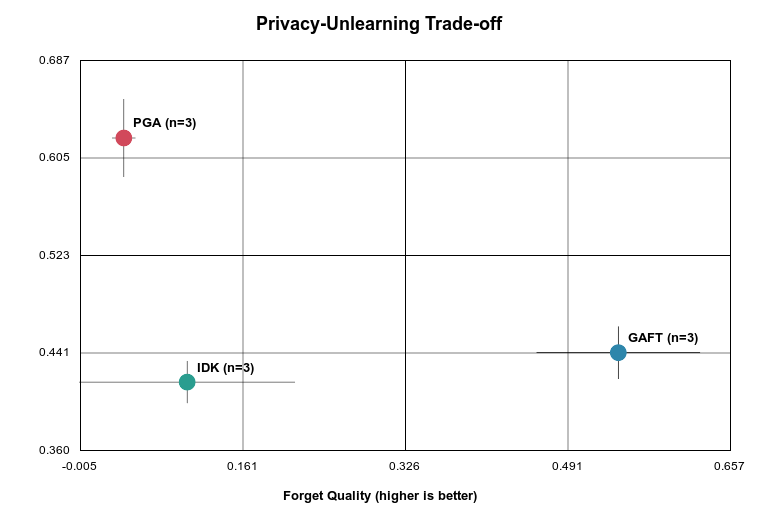
\includegraphics[width=\columnwidth]{analysis/generated/tradeoff_scatter.png}
\caption{Privacy-unlearning trade-off aggregated across three seeds. Points denote seed-averaged method performance and error bars denote approximate 95\% confidence intervals across runs. GAFT achieves the best Forget Quality, while IDK achieves the lowest mean MIA score.}
\label{fig:tradeoff_scatter}
\end{figure}

\begin{figure}[htbp]
\centering
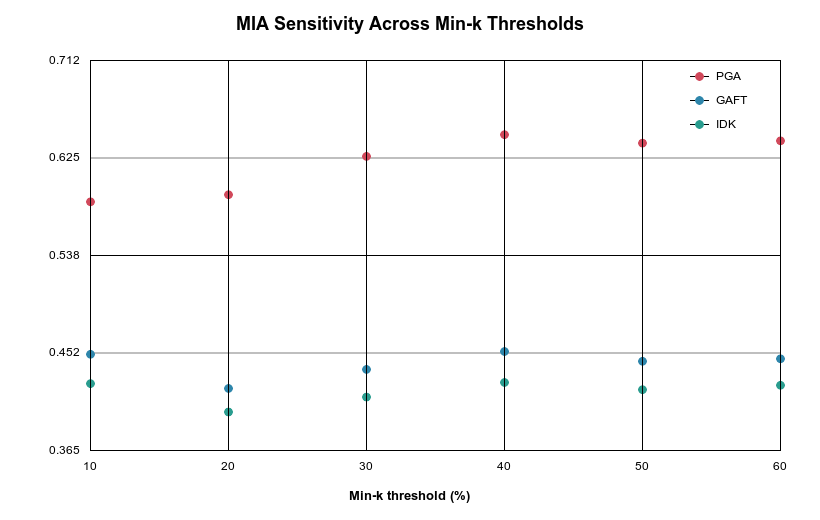
\includegraphics[width=\columnwidth]{analysis/generated/mia_thresholds.png}
\caption{MIA sensitivity across Min-$k$\% thresholds aggregated across three seeds. IDK remains consistently below GAFT and PGA across all six thresholds on average, indicating a stable privacy advantage under this attack family.}
\label{fig:mia_thresholds}
\end{figure}

\section{Discussion and Limitations}
\subsection{Discussion}
The implementation details in our notebooks help explain why the three methods occupy different points in the dependability trade-off space. PGA applies a direct sign-flip objective ($\mathcal{L}=-\mathcal{L}_{\mathrm{CE}}$) on forget10 only. This gives it the simplest optimization objective, but it also leaves the method without an explicit mechanism for preserving non-target behavior. In our evaluated 4-bit pipeline, this corresponds to the weakest aggregate profile under multi-seed evaluation: PGA has the highest mean MIA score and the lowest mean Forget Quality. The practical implication is not that pure ascent is universally ineffective, but that it appears under-constrained for dependable deployment under the current low-resource setting.

GAFT adds exactly the constraint that PGA lacks: every update jointly incorporates a forgetting signal and a retain-preservation signal through the mixed objective and fixed mixed-batch sampler. In our experiments, this produces the strongest overall behavior across the three evaluation axes and preserves the same qualitative ranking across seeds. GAFT is the only method that simultaneously attains high Forget Quality, substantially reduced MIA relative to PGA, and the strongest cross-split utility profile. This makes GAFT the clearest evidence in the paper that objective design matters more than aggressive forgetting alone when unlearning is evaluated from a deployment perspective.

IDK tuning reveals a different unlearning mode. Its lower forget accuracy, lower forget ROUGE-L, and lowest MIA scores indicate that target replacement is effective at suppressing direct recall and reducing attack exposure. However, the generated outputs also show that IDK does not always produce a clean abstention behavior. In several forget examples, the model responds with fabricated substitute biographies or drifts into unrelated continuations rather than consistently answering with a stable refusal. This qualitative failure mode is meaningful for DSML because it shows that low answer overlap is not equivalent to trustworthy deletion behavior. A model may stop reproducing the original fact while still generating confident hallucinated content about the same entity, which weakens the security interpretation of purely overlap-based metrics.

Across all three methods, the training backbone is intentionally controlled: the same 4-bit base model (\texttt{unsloth/llama-3-8b-bnb-4bit}), the same LoRA configuration ($r=16$, $\alpha=16$, same target modules, rank-stabilized LoRA enabled), and closely matched optimization settings (AdamW 8-bit, linear scheduler, gradient accumulation of 4, batch size 2, seeds 3407/3408/3409). This controlled setup increases the credibility of the comparison because the observed differences are much more plausibly explained by the unlearning objectives than by confounding implementation changes.

Taken together, the findings suggest that unlearning effectiveness cannot be evaluated in isolation from deployment conditions. In particular, low-bit quantization should be treated as part of the threat and reliability model rather than as a purely efficiency-oriented implementation detail. From a dependable ML perspective, targeted unlearning should therefore be assessed using at least three complementary lenses: direct suppression on forget examples, retained utility on non-target examples, and privacy leakage under attack-oriented post hoc evaluation such as MIA. More broadly, the findings connect to DSML concerns around dependable generative AI, privacy/accountability in ML systems, benchmark design, and robustness analysis for deployed foundation-model pipelines.

\subsection{Limitations}
Several limitations follow directly from the current code and experimental protocol:
\begin{itemize}
\item \textbf{Single-model, single-quantization setting.} All experiments use one base model family and 4-bit loading only. Results may not transfer directly to other model scales, architectures, or quantization schemes.
\item \textbf{Single data configuration.} Unlearning is evaluated on TOFU \texttt{forget10}/\texttt{retain90} only. The conclusions may shift under other forget ratios or domain distributions.
\item \textbf{Limited hyperparameter exploration.} Key choices are fixed in code (e.g., GAFT $\gamma=0.7$, unlearning max\_steps=300, one retain-sampling ratio for IDK), so reported outcomes should be interpreted as strong baselines rather than global optima.
\item \textbf{Limited repeated-run evidence.} We now report three-seed aggregates, which materially improves robustness over a single-run protocol, but the number of runs is still modest. Stronger statistical claims about ranking stability would benefit from additional seeds.
\item \textbf{Evaluation pipeline assumptions.} The MIA evaluation uses a specific min-$k$\% feature design and SVC configuration; alternative attack models may produce different absolute leakage estimates.
\item \textbf{Prompt-format sensitivity.} The training/evaluation prompt templates are fixed (``\#\#\# Question/\#\#\# Answer'' with \texttt{if\_llama=False}); conclusions may vary under other prompting or instruction formats.
\item \textbf{No post-unlearning recovery tests.} The current notebooks report direct post-unlearning metrics, but do not yet include adversarial relearning, re-quantization stress tests, or stronger adaptive attacks.
\end{itemize}

More broadly, no single metric fully characterizes forgetting in LLMs; accordingly, our evaluation should be read as a practical multi-metric assessment rather than as proof of complete knowledge removal.

These limitations define a clear next-step agenda: broader model/quantization coverage, larger-scale repeated-run evaluation, systematic hyperparameter sweeps, and stronger post-unlearning robustness evaluations.

\section{Conclusion}
This work studies targeted unlearning in a realistic 4-bit quantized LLaMA-3 pipeline and shows that deployment constraints materially affect how unlearning methods should be judged. Under a three-seed evaluation protocol, the experiments support a three-way interpretation rather than a single universal winner. GAFT provides the strongest overall balance between forgetting efficacy, retained utility, and privacy leakage in the evaluated setting. IDK most aggressively suppresses direct recall and achieves the lowest MIA scores, but with a sharper utility cost and a less reliable abstention behavior. PGA is the weakest baseline in our setup, suggesting that unconstrained ascent is not a dependable default under low-resource quantized deployment conditions.

A second takeaway is conceptual: in LLMs, forgetting should be interpreted operationally rather than as unverifiable perfect semantic erasure. A model may reduce answer overlap on the forget set while still exposing residual membership signals or producing hallucinated substitutes, which is why evaluation should jointly consider forget-set suppression, retained functionality, and privacy-oriented attacks. Although our study remains limited to one model family, one quantization setting, and one TOFU configuration, the move from a single-seed to a three-seed protocol narrows the gap between idealized unlearning research and realistic deployment pipelines. We hope this encourages broader multi-seed, multi-model, and post-unlearning robustness evaluations for practical LLM unlearning.

\section*{References}
\begin{thebibliography}{00}
\bibitem{b1} Y. Yao \emph{et al.}, ``Large language model unlearning,'' in \emph{Advances in Neural Information Processing Systems (NeurIPS)}, 2023. [Online]. Available: \url{https://arxiv.org/abs/2310.10683}
\bibitem{b2} T. Gu \emph{et al.}, ``MEOW: Memory supervised LLM unlearning via inverted facts,'' 2024. [Online]. Available: \url{https://arxiv.org/abs/2409.11844}
\bibitem{b3} S. Koundinya \emph{et al.}, ``Machine unlearning in large language models,'' 2024. [Online]. Available: \url{https://arxiv.org/abs/2402.00751}
\bibitem{b4} X. Xu \emph{et al.}, ``OBLIVIATE: Robust and practical machine unlearning for LLMs,'' 2025. [Online]. Available: \url{https://arxiv.org/abs/2505.04416}
\bibitem{b5} J. Xu \emph{et al.}, ``LLM-Eraser: Adaptive prompt tuning for unlearning,'' 2024. [Online]. Available: \url{https://arxiv.org/abs/2404.11056}
\bibitem{b6} B. W. Lee \emph{et al.}, ``Distillation robustifies unlearning,'' 2025. [Online]. Available: \url{https://arxiv.org/abs/2402.00751}
\bibitem{b7} R. Shokri \emph{et al.}, ``Membership inference attacks against machine learning models,'' in \emph{Proc. IEEE Symposium on Security and Privacy}, 2017. [Online]. Available: \url{https://arxiv.org/abs/1610.05820}
\bibitem{b8} N. Carlini \emph{et al.}, ``Extracting training data from large language models,'' in \emph{USENIX Security Symposium}, 2021. [Online]. Available: \url{https://arxiv.org/abs/2012.07805}
\bibitem{b9} E. Hu \emph{et al.}, ``LoRA: Low-rank adaptation of large language models,'' 2021. [Online]. Available: \url{https://arxiv.org/abs/2106.09685}
\bibitem{b10} C. Ding \emph{et al.}, ``Unified parameter-efficient unlearning for LLMs,'' in \emph{International Conference on Learning Representations (ICLR)}, 2024. [Online]. Available: \url{https://arxiv.org/abs/2402.00751}
\bibitem{b11} D. Kalajdzievski, ``Scaling laws for forgetting in LLMs,'' 2024. [Online]. Available: \url{https://arxiv.org/abs/2401.05605}
\bibitem{b12} Z. Zhang \emph{et al.}, ``Catastrophic failure of LLM unlearning via quantization,'' in \emph{International Conference on Learning Representations (ICLR)}, 2024. [Online]. Available: \url{https://arxiv.org/abs/2402.03279}
\bibitem{b13} P. Maini \emph{et al.}, ``TOFU: A task of fictitious unlearning,'' 2024. [Online]. Available: \url{https://arxiv.org/abs/2401.06121}
\bibitem{b14} D. Han, M. Han, and Unsloth team, \emph{Unsloth}. 2023. [Online]. Available: \url{https://github.com/unslothai/unsloth}
\end{thebibliography}

\end{document}
